\documentclass{article}

\usepackage[utf8]{inputenc} % accents
\usepackage[T1]{fontenc}      % caractères français
\usepackage{geometry}         % marges
\usepackage[francais]{babel}  % langue
\usepackage{graphicx}         % images
\usepackage{verbatim}
\usepackage{url}
\bibliographystyle{alpha}

\title{Document d'analyse des besoins}
\author{Alexandre Casanova-Franger\\
        \and
        Gauthier Lamarque\\
        \and
        Paul Simorre\\
        \and
        Lucas Vivas\\}

\begin{document}
  \maketitle
  \section{Introduction}
    \paragraph{}
    Ce projet consiste à améliorer un outil informatique d'analyse sonore dans
    l'optique de faciliter l'improvisation musicale. À terme, cet outil aura pour
    objectif de permettre à des musiciens de pouvoir améliorer leur
    improvisation. De plus, cet outil aura une portée scientifique, dans le sens
    où il sera possible d'étudier l'adaptation des musiciens grâce aux retours
    fournis par l'outil. \\
    Cet outil est basé sur une plateforme externe appelée Bela \cite{BELA},
    qui est un système embarqué de traitement audio en temps réel.
  \section{Description et analyse de l'existant}
    \paragraph{}
    À ce jour, l'outil est capable de fournir une représentation graphique de la
    corrélation des entrées audio. La corrélation est une notion centrale
    concernant cet outil. La corrélation est en fait une relation statistique
    entre deux ou plusieurs variables, et dans notre cas, il s'agit de la
    relation entre deux échantillons audio.
    \paragraph{}
    Les entrées audio sont gérées par le système embarqué Bela, qui peut
    recevoir 8 entrées analogiques (par l'intermédiaire de micros), 2 entrées
    audio (par l'intermédiaire de prises Jack) et enfin la possibilité d'inclure
    des fichiers audio (de type wav).\\
    La mécanique principale du programme consiste à récupérer des échantillons
    provenant des entrées audio, de les stocker dans des buffers, et d'appliquer
    une fonction de calcul de corrélation sur chaque paire d'échantillons
    (échantillons correspondant à des entrées distinctes). Ces échantillons
    sonores sont représentés sous la forme de vecteurs de nombres flottants.\\
    De ce fait, le calcul de la corrélation prend en entrée deux vecteurs de
    nombres flottants et renvoie un nombre flottant compris entre 0 et 1.
    Dans l'état actuel de l'outil, le calcul de la corrélation correspond au
    produit scalaire des deux vecteurs de flottants passés en entrée. Cependant,
    grâce au fichier de configuration de l'outil, il est possible de modifier la
    méthode de calcul de cette corrélation.
    \paragraph{}
    Enfin, une fois les coefficients de corrélation sont calculés, ceux-ci sont
    affichés suivant une matrice de corrélation, où $x_{i,j}$ correspond au
    coefficient de corrélation entre l'entrée i et l'entrée j.\\
    Sachant cela, la matrice de corrélation obtenue est donc une matrice
    symétrique (où $x_{i,j} = x_{j,i}$) et la diagonale de celle-ci est égale à
    1 ($x_{i,i} = 1$).
  \section{Description des besoins}
    \subsection{Besoins fonctionnels}
    \paragraph{}
    \begin{itemize}
      \item Présenter un retour sonore à l'utilisateur à partir de la matrice de
      corrélation. Il pourra dépendre d'une configuration choisie par l'utilisateur.
      \item On pourra présenter un retour sonore en temps réel à l'utilisateur sous
      forme d'un métronome destiné aux artistes et qui s'adapte dynamiquement au son
      en entrée ; en prenant par exemple pour référence le tempo joué par le musicien
      dont la somme des indices de corrélation avec tous les autres musiciens du groupe
      est la plus haute.
      \item L'utilisateur pourra avoir une représentation graphique des niveaux
      sonores sous la forme d'une matrice, de la même manière que la matrice de
      corrélation.
      \item L'utilisateur aura à sa disposition une liste de configurations
      pré-établies, dont les suivantes :
      \begin{itemize}
        \item Augmenter le volume des paires d'entrées les plus corrélées
        \item Augmenter le volume des paires d'entrées les moins corrélées
        \item Augmenter le volume des entrées dont la somme des indices de
        corrélation avec toutes les autres entrées est la plus élevée...
      \end{itemize}
      \item L'utilisateur pourra ajouter une nouvelle configuration, suivant
      une signature donnée.
      \item L'utilisateur pourra changer la fenêtre temporelle de calcul de
      corrélation.
    \end{itemize}
    \subsection{Besoins non-fonctionnels}
    \begin{itemize}
      \item Les signatures des méthodes calculant les niveaux sonores des
      entrées devront être génériques de façon à permettre aux utilisateurs d'en
      ajouter de nouvelles.
      \item Le temps de latence du programme doit être inférieur à 1 seconde.
      En effet, la durée d'acquisition de données (delta t) sera de 1 seconde,
      donc si l'on veut donner un sortie audio en temps réel, il faut que la latence
      soit au maximum de 1 seconde.
    \end{itemize}
    \subsection{Scénarios, prototypes, diagrammes, etc.}
      \paragraph{}
      Nous allons décrire ci-après un scénario que nos clients ont imaginé :\\
      L'utilisateur utilise l'outil sur un groupe de musiciens. Des micros sont
      branchés sur les différentes entrées analogiques et chaque musicien dispose
      d'un retour son. L'utilisateur configure le fichier de configuration afin
      que les paramètres décrits ci-dessus soient correctement pris en compte
      par l'outil. Les musiciens se mettent à improviser comme bon leur semble,
      et l'on peut observer en temps réel les corrélations entre les différents
      musiciens. On pourra aussi observer une matrice dite de "mixage" qui
      affiche les différents poids des paires de musiciens en fonction d'une
      configuration par défaut. À tout moment, l'utilisateur peut choisir une
      configuration de mixage différente pour que le retour sonore change.\\
      L'intérêt est d'étudier comment les musiciens s'adaptent en fonction du
      retour sonore, donc en fonction de la configuration de mixage choisie.
  \section{Diagramme de Gantt}
    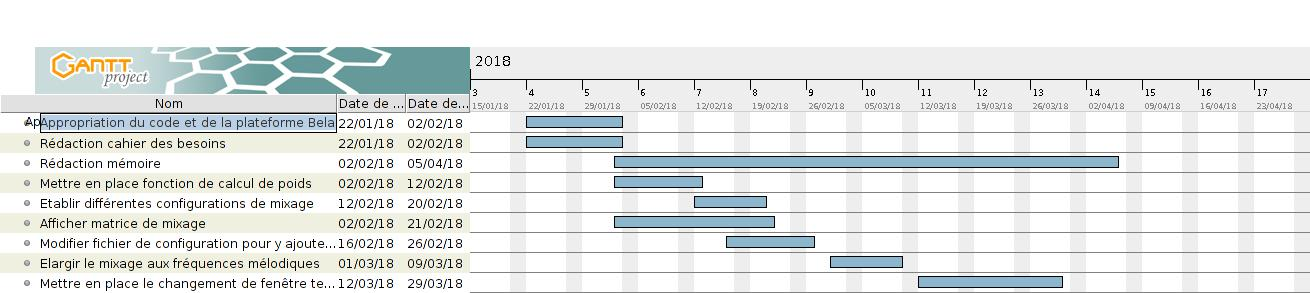
\includegraphics[scale=0.35]{DiagrammeAnalyseBesoins.jpg}
  \bibliography{analyse-besoins}
\end{document}
